\section{Overview}
\label{sec:motivation}
% Contemporary host PIDS, exemplified by \unicorn~\cite{han2020unicorn}, \streamspot~\cite{streamspot}, \threatrace~\cite{wang2022threatrace} and \prographer~\cite{yangprographer}, heavily rely on system audit log data to identify malicious entities within a system. Employing advanced deep learning techniques such as \gnn (\gnnshort), these systems strive to enhance the accuracy of threat detection. However, the efficacy of these techniques is contingent upon vast amounts of data to train the underlying models, often reaching terabytes in size. Acquiring such extensive training data from a single user machine is impractical.

% Our investigation, involving the simulation of normal user workloads on test machines, reveals that the audit logs generated from these activities are relatively small in volume. Consequently, they prove insufficient for adequately training these large-scale machine learning models. To address this limitation, it becomes imperative to aggregate data from a diverse array of machines to a centralized storage system for comprehensive model training.

% Nevertheless, the consolidation of audit logs from various sources poses a significant challenge due to the inherent risk of privacy leakage. These logs contain vital information about the diverse activities carried out by different users, encompassing details about utilized applications, browsing history, and sensitive data like email content, phone numbers, as well as financial and medical information. These privacy concerns are underscored in a report by Datadog~\cite{datadog}, a prominent provider of system monitoring services. Consequently, utilizing existing systems for detecting system threats introduces a potential compromise of user privacy.

% Moreover, the centralized aggregation of all data elevates the risk of data leakage and compromises the efficiency of these systems in terms of both memory utilization and runtime efficiency. As a result, there is a pressing need for innovative solutions that balance the imperative of robust threat detection with the paramount importance of safeguarding user privacy and system efficiency.

% Federated learning (FL) is an establish technique for privacy preserving machine learning. In federated learning the individual client data does not leave the system. Instead each client machine trains a local machine learning model on its local data and then these clients sends the trained model to a central server where the federated averaging is utilized to combine the information from these models to get a unified global model. However our experimentation with existing systems reveal that applying federated learning to them yields poor results because these systems are not designed to work in this fashion.

%\wajih{make a macro for Provenance-based IDS which is PIDS and use PIDS everywhere where you say intrusion detection. It saves space and also narrows the scope of our paper to PIDS. Use macros for words like word2vec, etc. because of letter capitalization. Also convert the words like Graph Neural Network into GNN to save space.}

\subsection{Background: Data Provenance Graphs}
%\wajih{citations are missing in this subsection.}
%\wajih{Add one or two paragraphs explaining provenance graphs. Give information about what is present in audit logs. Provide information about how to convert audit logs into provenance graphs. }

\begin{figure}[t!]
  \centering
  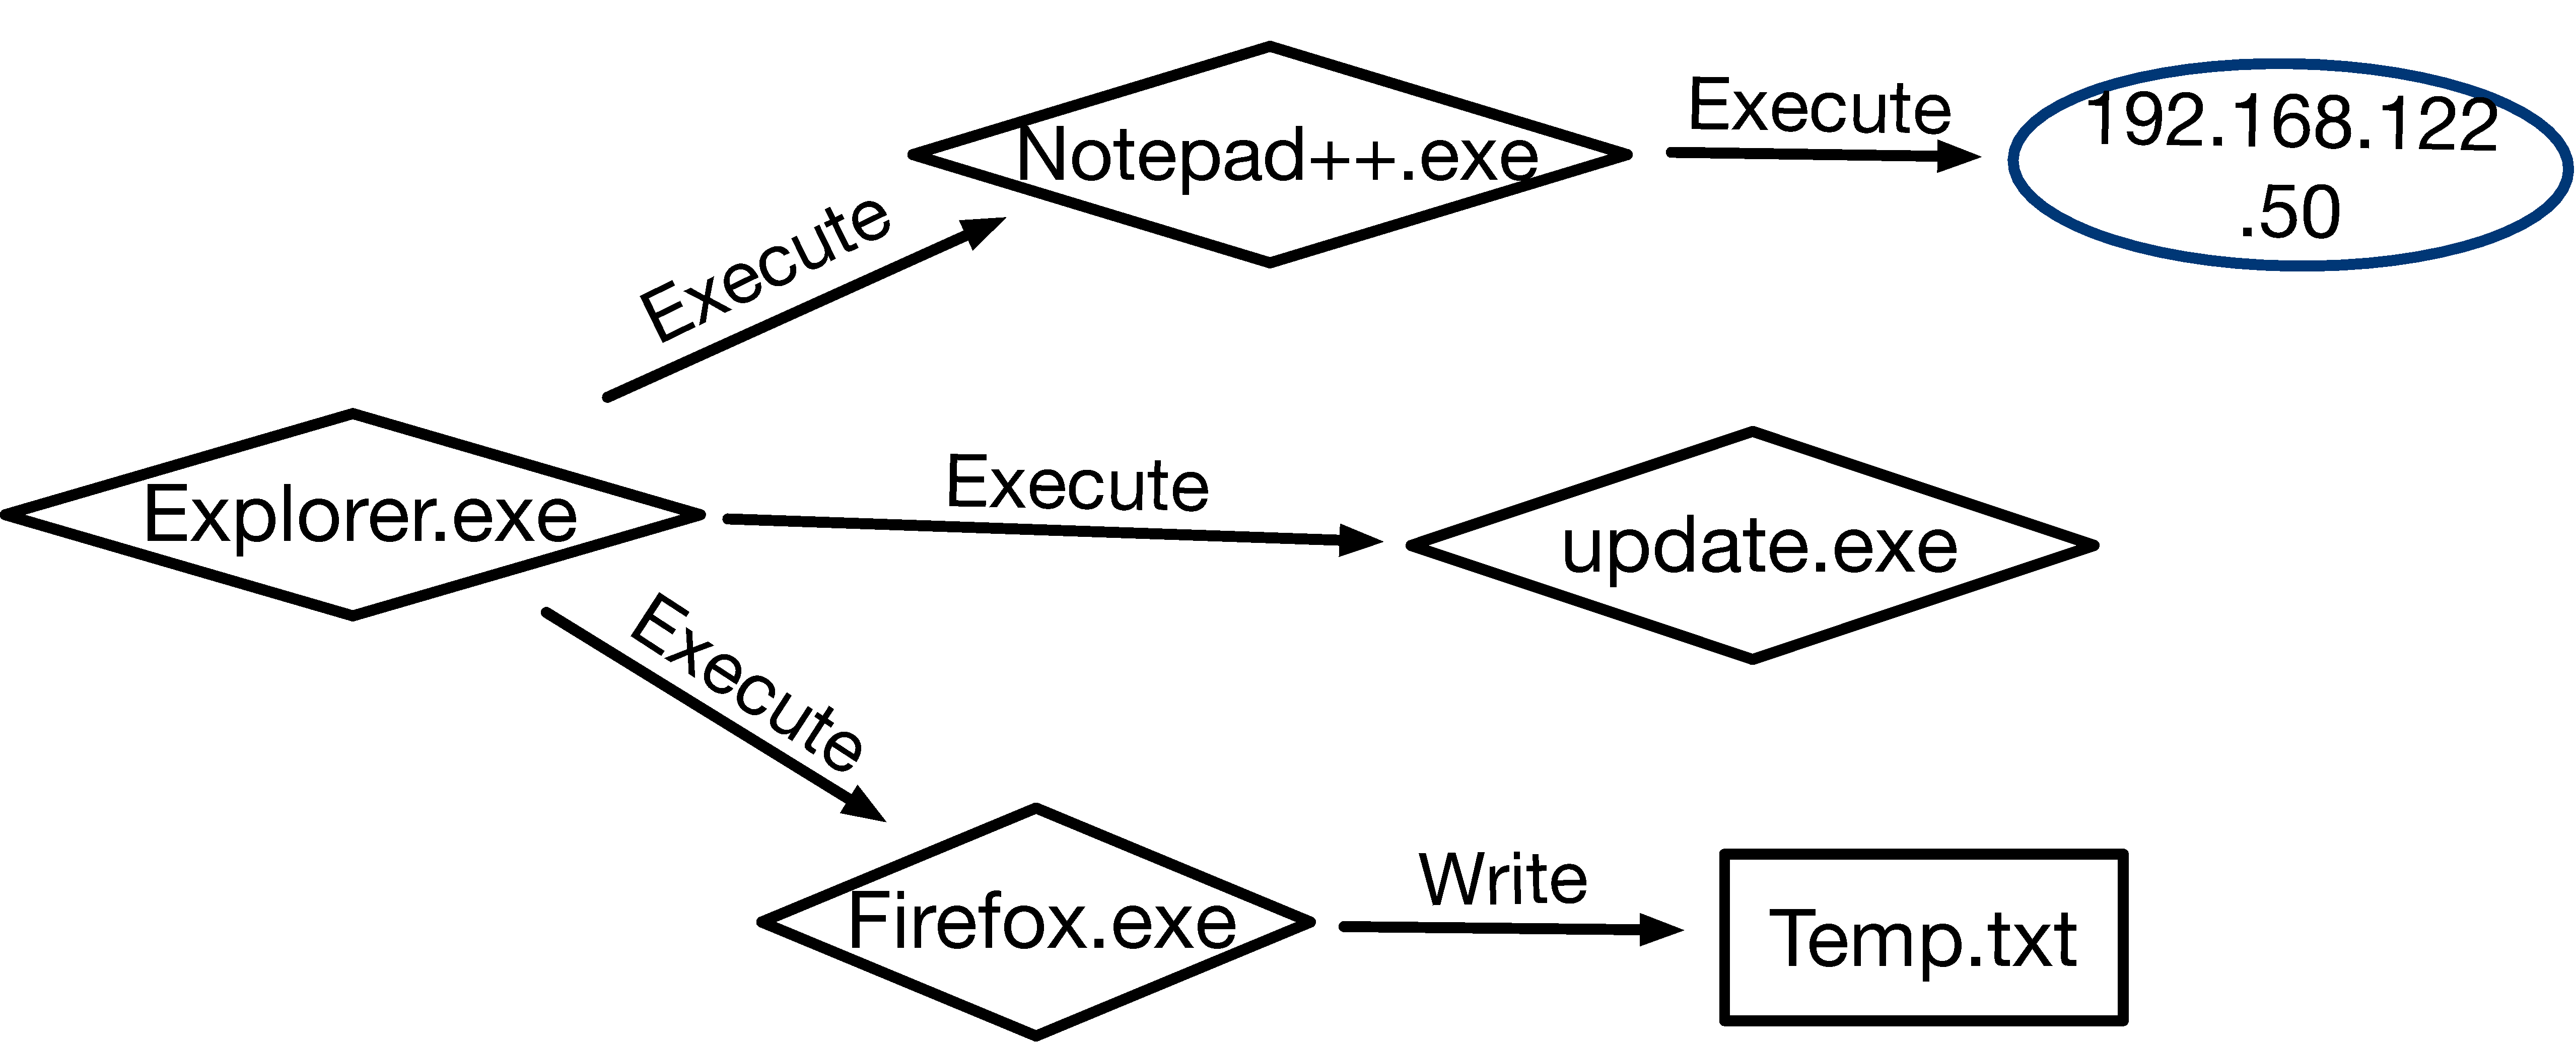
\includegraphics[width=0.4\textwidth]{fig/provexp.pdf}
  \caption{Data provenance graph example.}

  \label{provexp}
  \vspace{-2ex}
\end{figure}

%\wajih{Please put a concise provenance graph figure here.}

\Logs play a crucial role in recording the activities within a system, detailing interactions among various system entities such as processes, files, and sockets. Various operating systems come equipped with built-in mechanisms to gather these logs, including Event Tracing for Windows (ETW)~\cite{windowsaudit}, the Linux Audit system~\cite{linuxaudit}, and DTrace~\cite{dtrace} for FreeBSD. Each entry in a \logs characterizes a system event, identifying a subject and an object entity within the system. Moreover, these records include additional contextual attributes, including process names, file names, and socket IP addresses.

Data provenance employs the concept of modeling the causal links among different system entities. Fundamentally, it utilizes system logs to construct a dependency graph that captures the relationships between events. Within this graph, nodes symbolize system entities such as processes, files, and sockets, while the edges represent various system syscalls. This provenance graph is instrumental in analyzing the activities of different system entities and plays a vital role in identifying anomalous or malicious entities. Figure~\ref{provexp} shows an example of a provenance graph where \textit{Explorer.exe} is executing other processes such as \textit{Notepad.exe} and \textit{Firefox.exe}. These processes then interact with other file and socket nodes.

%\wajih{Since we do not have any provenance graph in the paper, we need to provide a short example of a provenance graph.}


% \subsection{Provenance-based IDS (PIDS)}
% Provenance-based Intrusion Detection Systems can be broadly classified into two main types: rule-based and learning-based approaches. The rule-based approaches~\cite{holmes2019,rapsheet2020,poirot2019} leverage knowledge of known attack behaviors to identify attack activities in the provenance graph. However, developing these rules demands significant effort from analysts, and attacks with unseen patterns could go undetected. Conversely, learning-based approaches~\cite{wang2022threatrace,flash2024,cheng2023kairos,yangprographer,shadewatcher} focus on detecting zero-day attacks without requiring prior knowledge of past attacks or specific rules. These anomaly-based methods establish a baseline of benign system activities and identify any significant deviations from this baseline behavior as anomalies.

% \subsection{Limitations of Existing PIDS}
% Here we examine existing PIDS and underscore their design flaws, particularly regarding the preservation of user log privacy and scalability. \flash~\cite{flash2024}, a node-level anomaly detection system, utilizes Graph Neural Networks to learn standard system behavior from provenance graphs. This system adopts an advanced featurization method, using a temporal ordering-aware \wordvec model to capture both structural and semantic characteristics in \logs. Moreover, \flash enhances inference speed via a \gnnshort embedding store. In contrast, \threatrace~\cite{wang2022threatrace}, another node-level detection system, also employs Graph Neural Networks for anomaly detection. However, it stands apart from \flash due to its scalability issues and reliance on basic features, which limits its effectiveness in fully leveraging the information contained in provenance graphs. \kairos~\cite{cheng2023kairos}, an anomaly-based detector, segments logs into time window queues and uses temporal graph neural networks for anomaly detection. Despite the progress made by existing PIDS, they fail to provide any privacy safeguards for sensitive information that may be contained in the \logs they utilize. This deficiency can impede the deployment of these systems in real world settings.

% We provide three limitations of existing systems in detail in Section~\ref{s:intro}, namely: lack of privacy preservation, excessive network overhead, and limited scalability. Table~\ref{tab:limitations} provides an overview of the limitations of existing systems.


% \PP{Lack of Privacy Preservation} The existing PIDSes that have been discussed above predominantly rely on system log data to identify malicious entities within a system. These systems employ advanced deep learning techniques, such as \gnn, to achieve impressive detection results. However, a notable downside of these models is their substantial requirement for data to accurately learn benign system behavior. This volume of data is impracticable to generate from a single user's machine. Consequently, in an enterprise environment, it becomes essential to collect data from a multitude of machines in order to compile a sufficiently large dataset for training these detection systems.  We conducted experiments with the \flash system by training it on data from a single host from \optc and compared the results with those reported in their paper, which were generated using data from multiple hosts. We observed a significant decrease in detection performance when using data from a single host, with the F-score experiencing a 40\% reduction.

% The centralized approach introduces a significant risk to user privacy. When a central entity analyzes these logs, it gains insights into the users system activities. This can range from identifying the applications they use, to the websites they browse, and even potentially inferring their location from network IPs. Thus, while existing PIDS are effective in identifying system threats, they simultaneously pose a potential compromise to user privacy.

% \PP{Excessive Network Overhead} The current systems function under the premise of a centralized infrastructure designed for aggregating user logs to train models. In this setup, user machines periodically transmit their logs to a central server, which then consolidates them in a centralized database. However, the volume of these log data can reach gigabytes, resulting in significant network expenses for both users and the organization. Such extensive network costs disproportionately affect users with limited bandwidth, as they may be unable to contribute their data for model training. This exclusion hampers the model's ability to learn a comprehensive representation of benign behavior, potentially leading to a higher rate of false alarms for those not participating. Our analysis of the \optc dataset reveals that each host generates approximately 1 GB of log data daily. In a real-world enterprise with hundreds of users, this translates to several hundred gigabytes of data being transmitted to the server each day for threat detection. Such volumes pose significant infrastructure and scalability challenges for centralized detection systems.

% \PP{Limited Scalability} The existing systems train their deep neural models using logs stored centrally. This approach significantly prolongs the training time of the models. The challenge escalates when frequent retraining is required to address the issue of concept drift~\cite{lu2018learning}. Additionally, these systems lack inherent mechanisms for parallelizing the training process. Moreover, since all logs need to be aggregated in a centralized storage, the disk overhead costs for the organization increase. The necessity for extensive disk storage can restrict organizations from incorporating data from all users, which might introduce data bias and degrade the model's performance in practical scenarios for these clients.

% Although existing systems, such as \flash, have implemented techniques to achieve efficient runtime performance. However, in an enterprise context, the centralized mode of operation faces scalability limitations. It can only accommodate a fixed number of hosts before the central server, running the intrusion detection system, becomes a bottleneck leading to log congestion. In high-throughput environments, this leads to the detector suffering from log congestion.

% \begin{table}[t!]
%     \centering
%     \scriptsize
%       %\caption{Limitations of existing PIDS. \wajih{Add in caption that which PIDS are not specified in the table and why.}}
%       \caption{Existing PIDS limitations: \flash and \kairos outperform other existing PIDS systems ~\cite{wang2022threatrace,han2020unicorn,streamspot,yangprographer,shadewatcher,provdetector2020}. Therefore, we have excluded these PIDS from the table.}
%       \setlength{\tabcolsep}{4.8pt}
%         \begin{tabular}{ | c | c | c | c | c |}
%           \hline
%                & \bf Privacy & \bf Network  & \bf Disk  & \bf Scalability \\
%                & \bf  Preserving & \bf  Cost & \bf Cost &  \\
%           \hline
%           \Sys  & YES                & LOW          & LOW       & HIGH        \\
%           \hline
%           \disdet~\cite{dong2023distdet} & NO                & LOW         & LOW      & HIGH       \\
%           \hline
%           \flash~\cite{flash2024}     & NO            & HIGH         & HIGH      & MEDIUM      \\
%           \hline
%           \kairos~\cite{cheng2023kairos}     & NO            & HIGH         & HIGH      & LOW         \\
%           \hline
%         \end{tabular}
%         \label{limitations}
%     \end{table}

\subsection{Background: Federated Learning}

Federated learning (FL)~\cite{mcmahan2017communication} is a machine learning approach that enables a model to be trained across multiple decentralized devices or servers holding local data samples, without exchanging them. This method addresses privacy concerns, bandwidth limitations, and data security issues inherent in centralized machine learning approaches used in existing PIDS~\cite{flash2024,cheng2023kairos,wang2022threatrace}. The mathematical formulation of FL involves aggregating locally computed updates to a global model, rather than directly sharing raw data.

In a federated learning setup, consider a global model parameterized by \(\theta\). The goal is to minimize some loss function \(L(\theta)\) that measures the discrepancy between the model's predictions and the actual data across all devices. However, instead of pooling all the data together, each device \(i\) computes an update \(\Delta \theta_i\) based on its local data and a local loss function \(L_i(\theta)\). Mathematically, the update rule on device \(i\) for a learning rate \(\eta\) is given by \(\Delta \theta_i = -\eta \nabla L_i(\theta)\), where \(\nabla L_i(\theta)\) is the gradient of the loss function with respect to the model parameters for the local data. After computing \(\Delta \theta_i\), each device sends this update to a central server.

The central server aggregates these updates from all participating devices to update the global model. The aggregation is an average function: \(\Delta \theta_{global} = \frac{1}{N} \sum_{i=1}^{N} \Delta \theta_i\), where \(N\) is the number of devices. This aggregated update is then used to update the global model parameters: \(\theta_{new} = \theta + \Delta \theta_{global}\). This process iterates, with the updated global model being sent back to the devices for further local updates, until convergence. This iterative process ensures that the global model learns from all devices while keeping the data localized, thus addressing privacy and bandwidth concerns.


\subsection{Why is it challenging to apply FL to \pids?}

Applying FL to PIDS can be challenging due to the heterogeneity of data across devices, which can lead to skewed model updates and performance variances. This is often referred to as non-IID~\cite{zhao2018federated} data, where the local data on each device may not represent the overall distribution of data across the organization. Additionally, applying FL to existing PIDS will produce suboptimal results. This is primarily because these systems were not originally designed to function under a federated learning framework. These challenges are discussed below:

\PP{Data imbalance \& heterogeneity among clients} In federated learning scenarios, data distribution and volume can significantly vary across participating devices or clients. This variability can lead to scenarios where some clients have extensive data representing a wide array of benign patterns, while others possess limited or skewed data sets. Such imbalances challenge the training of a global model that performs uniformly well across all clients, potentially causing the model to become biased towards clients with more comprehensive data collections. This bias may lead to the neglect of unique patterns found in less-represented clients. Existing PIDS lack built-in mechanisms to address this challenge effectively.

\PP{Feature space heterogeneity} \flash utilizes a temporally-aware Word2Vec model to encode the semantic attributes of entities within the provenance graph. In a federated learning environment, each client machine independently trains its Word2Vec model on its feature set. However, inherent randomness in the Word2Vec algorithm means that identical tokens may be encoded into different vectors by each client. Consequently, when federated averaging is applied to \gnn models that use these features, the performance is notably poor.

\PP{Temporal misalignment} \kairos leverages temporal graph neural networks to understand the evolution of a system's provenance graph over time. However, the application of federated learning to capture these temporal dependencies faces significant challenges. The fragmentation of data across various clients results in a lack of temporal alignment, which is crucial for the effectiveness of federated averaging in these network types. This misalignment impedes the ability to effectively integrate the learnings from individual client models into a cohesive global model.

\PP{Non-Privacy-Preserving data structure} \disdet employs a Hierarchical System Event Tree (HST) for storing the attributes of system events observed during the benign period. Events with attributes absent in the HST are subsequently identified as anomalous. This HST is forwarded to a central server, where attributes from HSTs of analogous clients are aggregated and redistributed. The architecture of the HST inherently precludes the possibility of preserving privacy. Furthermore, the reliance on a non-learning-based methodology restricts \disdet's capability to adapt to previously unseen benign patterns, making the application of machine learning algorithms, such as federated averaging~\cite{mcmahan2017communication}, unsuitable in this scenario.


\subsection{Overview of \Sys}
%\wajih{Lets use the word \fpgl throughout this paper. And say that we introduce the notion of \fpgl to solve the above challenges. Make sure you use this macro throughout the paper. }
The challenges outlined above significantly impede the adoption of federated learning in current systems. To overcome these hurdles, We introduce the notion of \fpgl , which integrates federated learning with \grl to create a privacy-preserving detection mechanism. Our approach introduces a novel framework that personalizes \grl at the system entity level, addressing data imbalance and client heterogeneity effectively.

To tackle feature space heterogeneity, we introduce a two-server architecture and an encryption scheme to privately synchronize individual semantic encoders across clients. Within this framework, each client trains an ensemble of \gnnshort models, with each model specializing in a particular category of system entities consistent across all participants. These models then participate in a federated averaging process coordinated by a central server. By specifying the learning objectives for each sub-model across clients, our method aims to standardize federated averaging, enhancing its robustness against skewed data distributions.

\Sys is composed of six key modules. The architecture begins with the \textit{Provenance Graph Constructor} module~\ref{provconstruct} on each client machine, transforming \logs into a provenance graph. Following this, the \textit{Semantic Featurization}~\ref{semanfeat} module encodes semantic attributes from the \logs into feature vectors, facilitating the training of client-specific \gnnshort models.

The \textit{Semantic Vectors Harmonization}~\ref{semanticharmonization} module aims to privately consolidate individual client word2vec models into a cohesive global model, employing a trusted utility server and encryption techniques to ensure the privacy of model data. Next, the \textit{Process Entity Categorization Module}~\ref{sys:catg} categorizes all system entities across clients into standardized categories, promoting uniformity in the training of \gnnshort models. The \textit{Federated Graph Learning Module}~\ref{sys:fpgl} proceeds to train \gnnshort models by these categories on each client machine, using the harmonized semantic features. After training, the models are sent to a central server for federated learning, where the federated averaging algorithm integrates the models based on the system entity categories they were trained on. Lastly, the \textit{Anomaly Detection Module}~\ref{sys:anomaly_detection} employs the unified global models for anomaly detection on each client machine. Figure \ref{fig:arch} presents the comprehensive architecture of \Sys, with further details in the subsequent subsections.

